% ROOT-G02 / L019-18: complete literal brace with its looped middle return.
% Manual source origin (600,1200), x right/y down, .008cm/source unit.
% Fixed rectangle (0,0)--(80,280), baseline local y140.
% Four draw commands preserve three visible runs; the last two meet at (48,172).
% No rendered or metric validation; surrounding aligned entries are outside this group.
\vcenter{\hbox{%
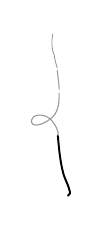
\begin{tikzpicture}[x=.008cm,y=-.008cm,baseline=(root-brace-base.base),line cap=round,line join=round]
\path[use as bounding box] (0,0) rectangle (80,280);
\node[anchor=base west,inner sep=0pt,outer sep=0pt] (root-brace-base) at (0,140) {};
\draw[gray!85,line width=.30pt] (40,10) .. controls (37,23) and (39,37) .. (42,43) .. controls (43,50) and (45,58) .. (47,64);
\draw[gray!75,line width=.40pt] (47,68) .. controls (48,78) and (50,90) .. (50,98);
\draw[gray!80,line width=.40pt] (50,104) .. controls (50,123) and (48,136) .. (36,145) .. controls (20,157) and (5,158) .. (6,147) .. controls (7,138) and (24,135) .. (36,145) .. controls (45,155) and (50,165) .. (48,172);
\draw[line width=.70pt] (48,172) .. controls (50,196) and (52,215) .. (57,233) .. controls (61,245) and (65,251) .. (66,257) .. controls (68,262) and (68,265) .. (64,267);
\end{tikzpicture}%
}}
